\documentclass[tikz, border=10pt]{standalone}
\usetikzlibrary{shapes.geometric, arrows.meta, positioning, calc}

\begin{document}

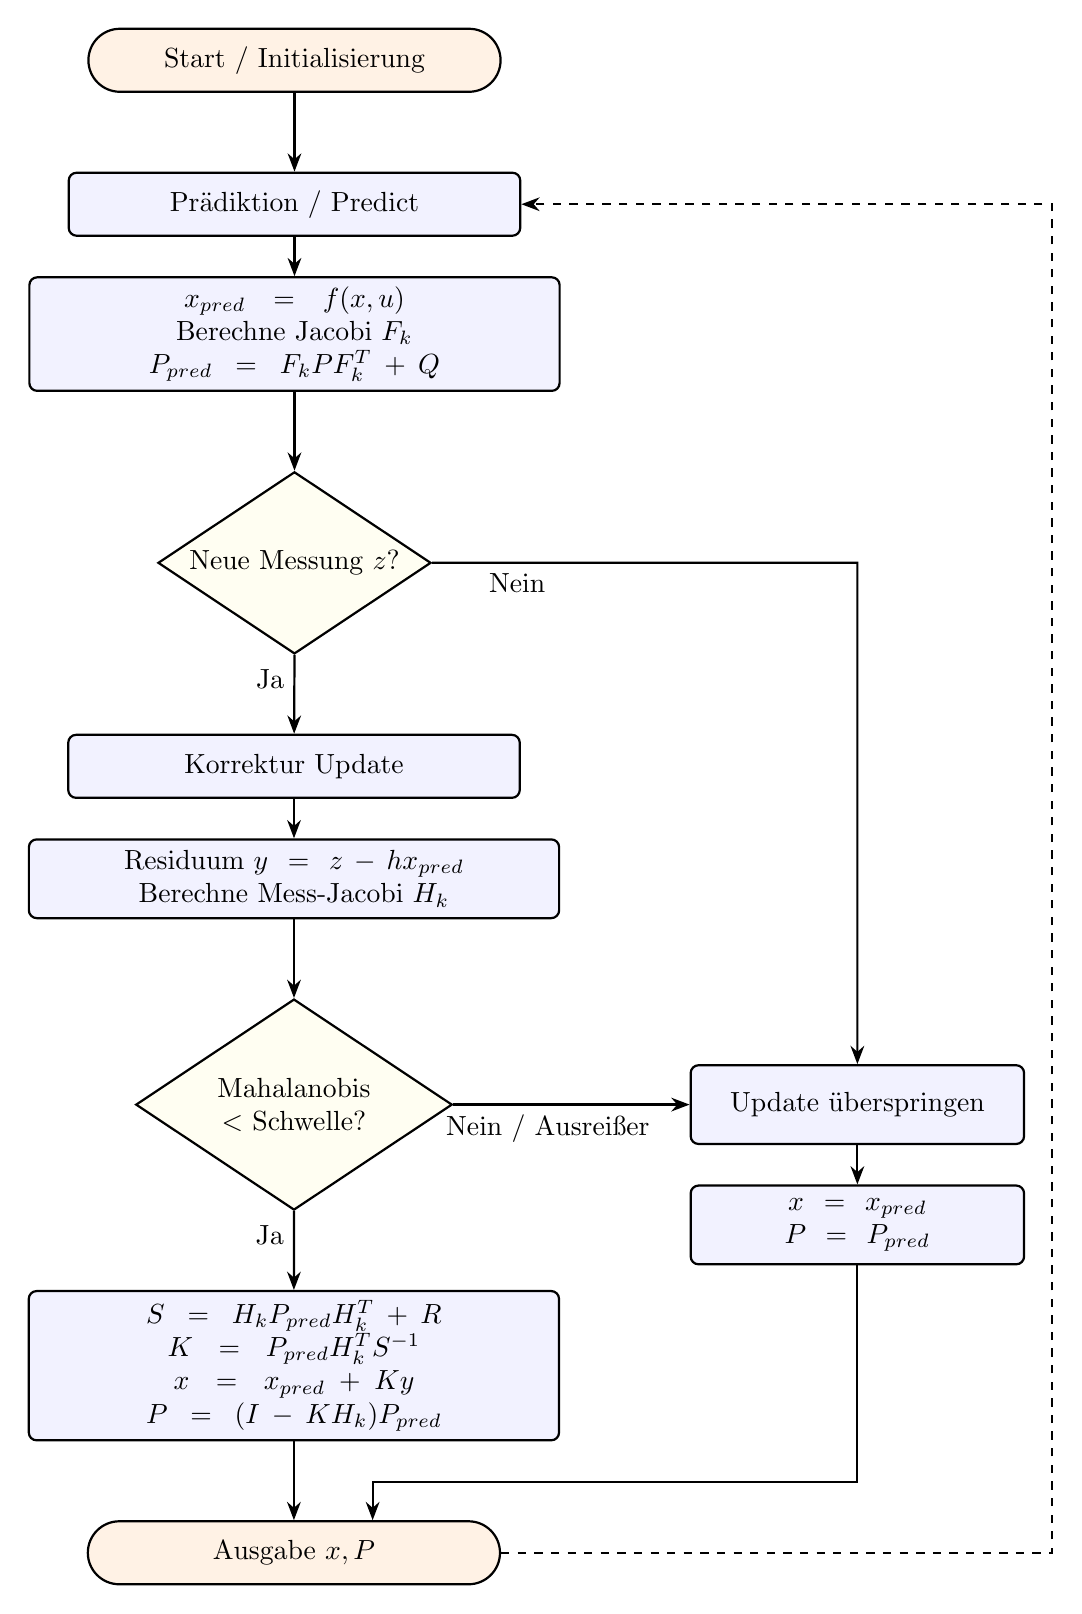
\begin{tikzpicture}[
    node distance=1.0cm and 1.5cm,
    auto,
    % --- STILDEFINITIONEN (MIT FARBEN) ---
    % Berechnungsschritte und Titel (Abgerundete Ecken, Blau)
    block_col/.style={
        rectangle, draw, thick, fill=blue!5, 
        rounded corners=0.1cm,
        text width=6.5cm, align=center, minimum height=1cm
    },
    % Titel-Blöcke (Kleiner, Blau)
    title_col/.style={
        rectangle, draw, thick, fill=blue!5, 
        rounded corners=0.1cm,
        text width=5.5cm, align=center, minimum height=0.8cm
    },
    % Spezialisierte Update-Blöcke (wie 'Skip', schmaler, Blau)
    skip_col/.style={
        rectangle, draw, thick, fill=blue!5, 
        rounded corners=0.1cm,
        text width=4cm, align=center, minimum height=1cm
    },
    % Entscheidungs-Rauten (Gelb)
    decision_col/.style={
        diamond, draw, thick, fill=yellow!5, 
        text width=3cm, align=center, inner sep=0pt, aspect=1.5
    },
    % Start & Ausgabe (Abgerundete Ecken, Orange)
    startstop_col/.style={
        rectangle, draw, thick, fill=orange!10, 
        rounded corners=0.4cm, text width=5cm, align=center, minimum height=0.8cm
    },
    % Pfeilstil
    line_style/.style={
        draw, -Stealth, thick
    }
]

% --- NODES ---

% Start
\node [startstop_col] (start) {Start / Initialisierung};

% Prädiktion
\node [title_col, below=of start] (predict_title) {Prädiktion / Predict};

\node [block_col, below=0.5cm of predict_title] (predict_eq) {
    $x_{pred} = f(x, u)$ \\
    Berechne Jacobi $F_k$ \\
    $P_{pred} = F_k P F_k^T + Q$
};

% Entscheidung Messung
\node [decision_col, below= of predict_eq] (new_meas) {Neue Messung $z$?};

% Korrektur Zweig (Ja)
\node [title_col, below left=1.0cm and -2.875cm of new_meas.south] (update_title) {Korrektur Update};

\node [block_col, below=0.5cm of update_title] (residuum) {
    Residuum $y = z - h x_{pred}$ \\
    Berechne Mess-Jacobi $H_k$
};

% Entscheidung Mahalanobis
\node [decision_col, below= of residuum] (maha_check) {Mahalanobis $<$ Schwelle?};

% Update Zweig (Ja)
\node [block_col, below left=1.0cm and -3.38cm of maha_check.south] (update_eq) {
    $S = H_k P_{pred} H_k^T + R$ \\
    $K = P_{pred} H_k^T S^{-1}$ \\
    $x = x_{pred} + K y$ \\
    $P = (I - K H_k) P_{pred}$
};

% Überspringen Zweig (Nein)
\node [skip_col, right=3cm of maha_check] (skip_title) {Update überspringen};

\node [skip_col, below=0.5cm of skip_title] (skip_eq) {
    $x = x_{pred}$ \\
    $P = P_{pred}$
};

% Ausgabe
\node [startstop_col, below= of update_eq] (output) {Ausgabe $x, P$};

% --- ARROWS ---

% Hauptfluss oben
\path [line_style] (start) -- (predict_title);
\path [line_style] (predict_title) -- (predict_eq);
\path [line_style] (predict_eq) -- (new_meas);

% Messung Entscheidung
\path [line_style] (new_meas.south) -- node[left, pos=0.3] {Ja} (update_title);
\draw [line_style] (new_meas.east) -- node[below, pos=0.2] {Nein} ++(5.4,0) -- (skip_title.north);

% Korrektur Fluss
\path [line_style] (update_title) -- (residuum);
\path [line_style] (residuum) -- (maha_check);

% Mahalanobis Entscheidung
\path [line_style] (maha_check.south) -- node[left, pos=0.3] {Ja} (update_eq.north);
\path [line_style] (maha_check) -- node[below, pos=0.4] {Nein / Ausreißer} (skip_title);

% Skip Fluss
\path [line_style] (skip_title) -- (skip_eq);

% Zusammenführung zur Ausgabe
\path [line_style] (update_eq.south) -- (output.north);%++(0,-0.5) -|
\draw [line_style] (skip_eq.south) -- ++(0,-2.75) -| ([xshift=1cm]output.north);

% Loop zurück zur Prädiktion (Gestrichelt, wie beim 1€-Filter)
\draw [line_style, dashed] (output.east) -- ++(7,0) |- (predict_title.east);

\end{tikzpicture}

\end{document}